\documentclass{article}\usepackage[]{graphicx}\usepackage[]{xcolor}
% maxwidth is the original width if it is less than linewidth
% otherwise use linewidth (to make sure the graphics do not exceed the margin)
\makeatletter
\def\maxwidth{ %
  \ifdim\Gin@nat@width>\linewidth
    \linewidth
  \else
    \Gin@nat@width
  \fi
}
\makeatother

\definecolor{fgcolor}{rgb}{0.345, 0.345, 0.345}
\newcommand{\hlnum}[1]{\textcolor[rgb]{0.686,0.059,0.569}{#1}}%
\newcommand{\hlstr}[1]{\textcolor[rgb]{0.192,0.494,0.8}{#1}}%
\newcommand{\hlcom}[1]{\textcolor[rgb]{0.678,0.584,0.686}{\textit{#1}}}%
\newcommand{\hlopt}[1]{\textcolor[rgb]{0,0,0}{#1}}%
\newcommand{\hlstd}[1]{\textcolor[rgb]{0.345,0.345,0.345}{#1}}%
\newcommand{\hlkwa}[1]{\textcolor[rgb]{0.161,0.373,0.58}{\textbf{#1}}}%
\newcommand{\hlkwb}[1]{\textcolor[rgb]{0.69,0.353,0.396}{#1}}%
\newcommand{\hlkwc}[1]{\textcolor[rgb]{0.333,0.667,0.333}{#1}}%
\newcommand{\hlkwd}[1]{\textcolor[rgb]{0.737,0.353,0.396}{\textbf{#1}}}%
\let\hlipl\hlkwb

\usepackage{framed}
\makeatletter
\newenvironment{kframe}{%
 \def\at@end@of@kframe{}%
 \ifinner\ifhmode%
  \def\at@end@of@kframe{\end{minipage}}%
  \begin{minipage}{\columnwidth}%
 \fi\fi%
 \def\FrameCommand##1{\hskip\@totalleftmargin \hskip-\fboxsep
 \colorbox{shadecolor}{##1}\hskip-\fboxsep
     % There is no \\@totalrightmargin, so:
     \hskip-\linewidth \hskip-\@totalleftmargin \hskip\columnwidth}%
 \MakeFramed {\advance\hsize-\width
   \@totalleftmargin\z@ \linewidth\hsize
   \@setminipage}}%
 {\par\unskip\endMakeFramed%
 \at@end@of@kframe}
\makeatother

\definecolor{shadecolor}{rgb}{.97, .97, .97}
\definecolor{messagecolor}{rgb}{0, 0, 0}
\definecolor{warningcolor}{rgb}{1, 0, 1}
\definecolor{errorcolor}{rgb}{1, 0, 0}
\newenvironment{knitrout}{}{} % an empty environment to be redefined in TeX

\usepackage{alltt}
\usepackage[sc]{mathpazo}
\renewcommand{\sfdefault}{lmss}
\renewcommand{\ttdefault}{lmtt}
\usepackage[T1]{fontenc}
\usepackage{geometry}
\geometry{verbose,tmargin=2.5cm,bmargin=2.5cm,lmargin=2.5cm,rmargin=2.5cm}
\setcounter{secnumdepth}{2}
\setcounter{tocdepth}{2}
\usepackage[unicode=true,pdfusetitle,
 bookmarks=true,bookmarksnumbered=true,bookmarksopen=true,bookmarksopenlevel=2,
 breaklinks=false,pdfborder={0 0 1},backref=false,colorlinks=false]
 {hyperref}
\hypersetup{
 pdfstartview={XYZ null null 1}}

\makeatletter
%%%%%%%%%%%%%%%%%%%%%%%%%%%%%% User specified LaTeX commands.
\renewcommand{\textfraction}{0.05}
\renewcommand{\topfraction}{0.8}
\renewcommand{\bottomfraction}{0.8}
\renewcommand{\floatpagefraction}{0.75}

\makeatother
\IfFileExists{upquote.sty}{\usepackage{upquote}}{}
\begin{document}








The results below are generated from an R script.

\begin{knitrout}
\definecolor{shadecolor}{rgb}{0.969, 0.969, 0.969}\color{fgcolor}\begin{kframe}
\begin{alltt}
\hlcom{# Assignment: ASSIGNMENT 4}
\hlcom{# Name: Reppeto, Brian}
\hlcom{# Date: 2023-06-27}

\hlcom{## Load the ggplot2 package}

\hlkwd{library}\hlstd{(tidyverse)}
\hlkwd{library}\hlstd{(readxl)}
\hlkwd{library}\hlstd{(ggplot2)}
\hlkwd{library}\hlstd{(dplyr)}
\hlkwd{library}\hlstd{(conflicted)}
\hlcom{#library(plyr)}
\hlkwd{theme_set}\hlstd{(}\hlkwd{theme_minimal}\hlstd{())}

\hlcom{## Set the working directory to the root of your DSC 520 directory}
\hlkwd{setwd}\hlstd{(}\hlstr{"~/DSC520/Week_4"}\hlstd{)}

\hlcom{## Load the `data` to}
\hlstd{housing_df} \hlkwb{<-} \hlkwd{read_xlsx}\hlstd{(}\hlstr{"week-6-housing.xlsx"}\hlstd{)}

\hlcom{#housing_df %>% rename("Sale_Price" = "Sale Price")}

\hlcom{#sum_by_day <-apply(housing_df$'Sale Price',housing_df$'Sale Date',sum)}


\hlcom{## 1.}
\hlstd{ttl_house_prices} \hlkwb{<-} \hlkwd{apply}\hlstd{(housing_df[}\hlkwd{c}\hlstd{(}\hlstr{'Sale Price'}\hlstd{)],} \hlnum{2}\hlstd{, sum)}

\hlkwd{print} \hlstd{(ttl_house_prices)}
\end{alltt}
\begin{verbatim}
## Sale Price 
## 8500391149
\end{verbatim}
\begin{alltt}
\hlcom{## 2.}
\hlstd{ttl_sales_by_zip} \hlkwb{<-} \hlkwd{aggregate}\hlstd{(`Sale Price`} \hlopt{~}  \hlstd{zip5,} \hlkwc{data} \hlstd{= housing_df, mean)}

\hlkwd{print} \hlstd{(ttl_sales_by_zip)}
\end{alltt}
\begin{verbatim}
##    zip5 Sale Price
## 1 98052   649375.4
## 2 98053   672623.7
## 3 98059   645000.0
## 4 98074   951543.8
\end{verbatim}
\begin{alltt}
\hlcom{## 3.}

\hlstd{housing} \hlkwb{<-}
  \hlkwd{rename}\hlstd{(housing_df,} \hlkwc{sale_price} \hlstd{= `Sale Price`,} \hlkwc{sale_date} \hlstd{= `Sale Date`)}

\hlstd{housing} \hlkwb{<-} \hlkwd{mutate}\hlstd{(housing,} \hlkwc{month} \hlstd{= lubridate} \hlopt{::} \hlkwd{month} \hlstd{(sale_date),}
                          \hlkwc{year} \hlstd{= lubridate} \hlopt{::} \hlkwd{year} \hlstd{(sale_date))}

\hlstd{sales_year} \hlkwb{<-} \hlkwd{aggregate}\hlstd{(sale_price} \hlopt{~} \hlstd{year,} \hlkwc{data} \hlstd{= housing, sum)}

\hlstd{housing} \hlkwb{<-} \hlkwd{mutate}\hlstd{(housing,} \hlkwc{sale_price_in_thous} \hlstd{= sale_price} \hlopt{/} \hlnum{1000}\hlstd{)}

\hlkwd{print}\hlstd{(sales_year)}
\end{alltt}
\begin{verbatim}
##    year sale_price
## 1  2006  919005546
## 2  2007  850285247
## 3  2008  755045696
## 4  2009  454417263
## 5  2010  592828305
## 6  2011  693256612
## 7  2012  747585171
## 8  2013  860712529
## 9  2014  792182425
## 10 2015  915474082
## 11 2016  919598273
\end{verbatim}
\begin{alltt}
\hlcom{## 4}
\hlkwd{ggplot}\hlstd{(housing,} \hlkwd{aes}\hlstd{(}\hlkwc{x} \hlstd{= sale_price_in_thous))} \hlopt{+}
  \hlkwd{geom_histogram}\hlstd{(}\hlkwc{fill} \hlstd{=} \hlstr{"lightblue"}\hlstd{,} \hlkwc{bins} \hlstd{=} \hlnum{30}\hlstd{)} \hlopt{+}
  \hlkwd{labs}\hlstd{(}\hlkwc{title} \hlstd{=} \hlstr{"Distribution of Sale Price in thousands"}\hlstd{)}
\end{alltt}
\end{kframe}

{\centering 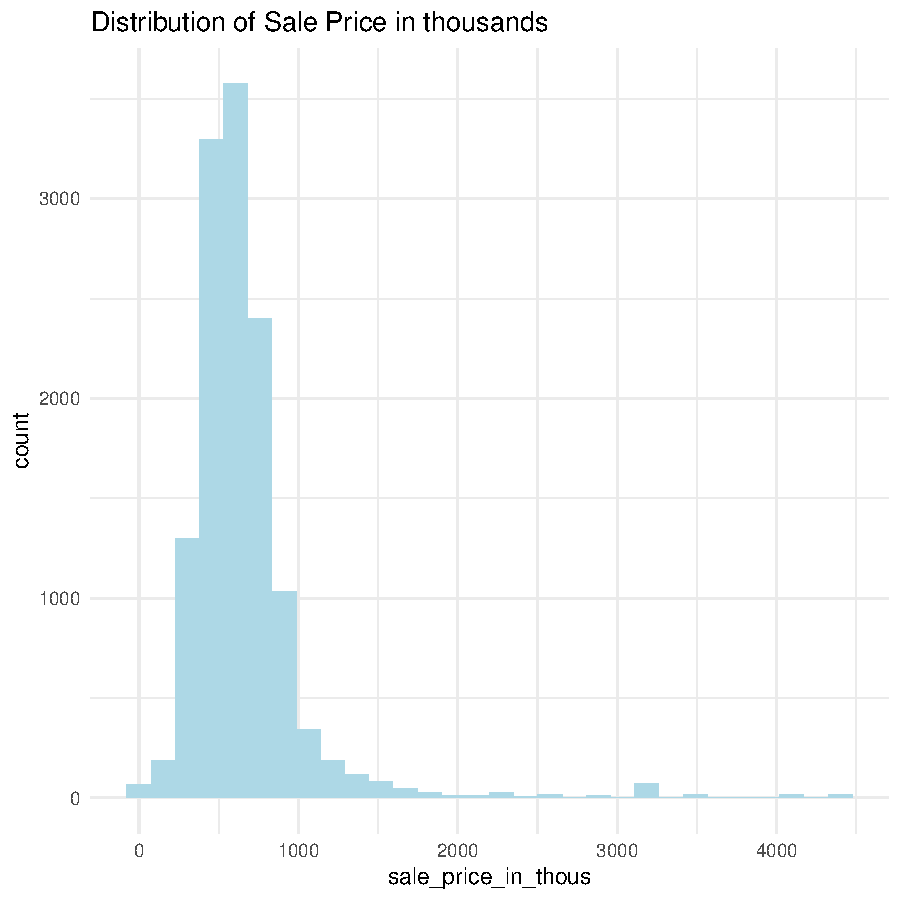
\includegraphics[width=.6\linewidth]{figure/assignment-04-Reppeto-Brian-Rnwauto-report-1} 

}


\begin{kframe}\begin{alltt}
\hlcom{## 5.}
\hlcom{## There are outliers in the data for the sale_price variable as shown in the}
\hlcom{## graph above.}

\hlcom{## 6.}
\hlstd{housing} \hlkwb{<-} \hlkwd{mutate}\hlstd{(housing,} \hlkwc{price_per_sf} \hlstd{=  sale_price}\hlopt{/}\hlstd{square_feet_total_living)}

\hlstd{housing} \hlkwb{<-} \hlkwd{mutate}\hlstd{(housing,} \hlkwc{commision} \hlstd{=} \hlnum{.06}\hlstd{)}

\hlstd{housing} \hlkwb{<-}
  \hlkwd{mutate}\hlstd{(housing,} \hlkwc{net_sales_price} \hlstd{= (sale_price} \hlopt{-} \hlstd{(sale_price} \hlopt{*} \hlstd{commision)))}

\hlcom{#head(select(housing,price_per_sf))                  }

\hlcom{#head(select(housing, net_sales_price, commision, sale_price_in_thous))}

\hlcom{##view(housing)}
\end{alltt}
\end{kframe}
\end{knitrout}

The R session information (including the OS info, R version and all
packages used):

\begin{knitrout}
\definecolor{shadecolor}{rgb}{0.969, 0.969, 0.969}\color{fgcolor}\begin{kframe}
\begin{alltt}
\hlkwd{sessionInfo}\hlstd{()}
\end{alltt}
\begin{verbatim}
## R version 4.3.0 (2023-04-21)
## Platform: aarch64-apple-darwin20 (64-bit)
## Running under: macOS Ventura 13.4.1
## 
## Matrix products: default
## BLAS:   /System/Library/Frameworks/Accelerate.framework/Versions/A/Frameworks/vecLib.framework/Versions/A/libBLAS.dylib 
## LAPACK: /Library/Frameworks/R.framework/Versions/4.3-arm64/Resources/lib/libRlapack.dylib;  LAPACK version 3.11.0
## 
## locale:
## [1] en_US.UTF-8/en_US.UTF-8/en_US.UTF-8/C/en_US.UTF-8/en_US.UTF-8
## 
## time zone: America/New_York
## tzcode source: internal
## 
## attached base packages:
## [1] stats     graphics  grDevices utils     datasets  methods   base     
## 
## other attached packages:
##  [1] conflicted_1.2.0 readxl_1.4.2     lubridate_1.9.2  forcats_1.0.0    stringr_1.5.0   
##  [6] dplyr_1.1.2      purrr_1.0.1      readr_2.1.4      tidyr_1.3.0      tibble_3.2.1    
## [11] ggplot2_3.4.2    tidyverse_2.0.0 
## 
## loaded via a namespace (and not attached):
##  [1] gtable_0.3.3     highr_0.10       compiler_4.3.0   tidyselect_1.2.0 scales_1.2.1    
##  [6] fastmap_1.1.1    R6_2.5.1         labeling_0.4.2   generics_0.1.3   knitr_1.43      
## [11] munsell_0.5.0    pillar_1.9.0     tzdb_0.4.0       rlang_1.1.1      utf8_1.2.3      
## [16] cachem_1.0.8     stringi_1.7.12   xfun_0.39        timechange_0.2.0 memoise_2.0.1   
## [21] cli_3.6.1        withr_2.5.0      magrittr_2.0.3   grid_4.3.0       rstudioapi_0.14 
## [26] hms_1.1.3        lifecycle_1.0.3  vctrs_0.6.3      evaluate_0.21    glue_1.6.2      
## [31] farver_2.1.1     cellranger_1.1.0 fansi_1.0.4      colorspace_2.1-0 tools_4.3.0     
## [36] pkgconfig_2.0.3
\end{verbatim}
\begin{alltt}
\hlkwd{Sys.time}\hlstd{()}
\end{alltt}
\begin{verbatim}
## [1] "2023-07-02 18:49:37 EDT"
\end{verbatim}
\end{kframe}
\end{knitrout}


\end{document}
